\chapter{Requisitos do Sistema}

Quando qualquer sistema é desenvolvido, este visa tornar possível diferentes casos de uso, sendo estes realizados por um ou mais atores.
Estes atores que interagem diretamente com o sistema possuem requisitos que o sistema tem que cumprir, isto é, funcionalidades que
o sistema tem que possuir de modo a poder responder às suas necessidades. Como tal, é necessário um levantamento destes requisitos, de modo
a melhor desenvolver o sistema para responder às necessidades dos seus utilizadores.

Deste modo, neste capítulo iremos não só apresentar os autores que irão interagir com o sistema, mas também os diversos usos que estes
utilizadores darão ao sistema, bem como os diversos requisitos que o mesmo tem de cumprir.

\section{Atores}

Como já foi referido, a criação de \emph{APIs GSMA Open Gateway} visa facilitar a utilização programática dos diversos recursos e
funcionalidades que a rede \emph{5G} consegue oferecer. Deste modo, o sistema possui 2 atores distintos.
\begin{itemize}
  \item \textbf{Operador de rede} - O primeiro ator a interagir com o sistema é o operador de rede,
    que fornece as APIs a diversos outros negócios para que estes possam interagir com a rede programáticamente. No entanto, tendo em
    consideração que as APIs desenhadas pelo \emph{GSMA Open Gateway} são consideravelmente mais simples que as definidas pelo \emph{3GPP},
    um operador de rede pode também utilizar estas APIs para gerir a própria rede.

  \item \textbf{Negócios clientes/Parceiros} - O segundo ator a interagir com o sistema é na realidade o seu público alvo. Diversos negócios
    que desenvolvem um conjunto de produtos que interagem com a rede. Estes negócios utilizaram as APIs definidas pelo \emph{GSMA Open Gateway}
    para não só oferecerem um maior leque de funcionalidades aos seus utilizadores, como também para fazer um conjunto de verificações, de modo
    a garantir a correta utilização e desempenho dos seus produtos.
\end{itemize}

\section{Casos de Uso}

Os dois atores apresentados na secção anterior possuem diversos casos de uso. Estes são apresentados no diagrama seguinte.

\begin{figure}[H]
  \centerline{
    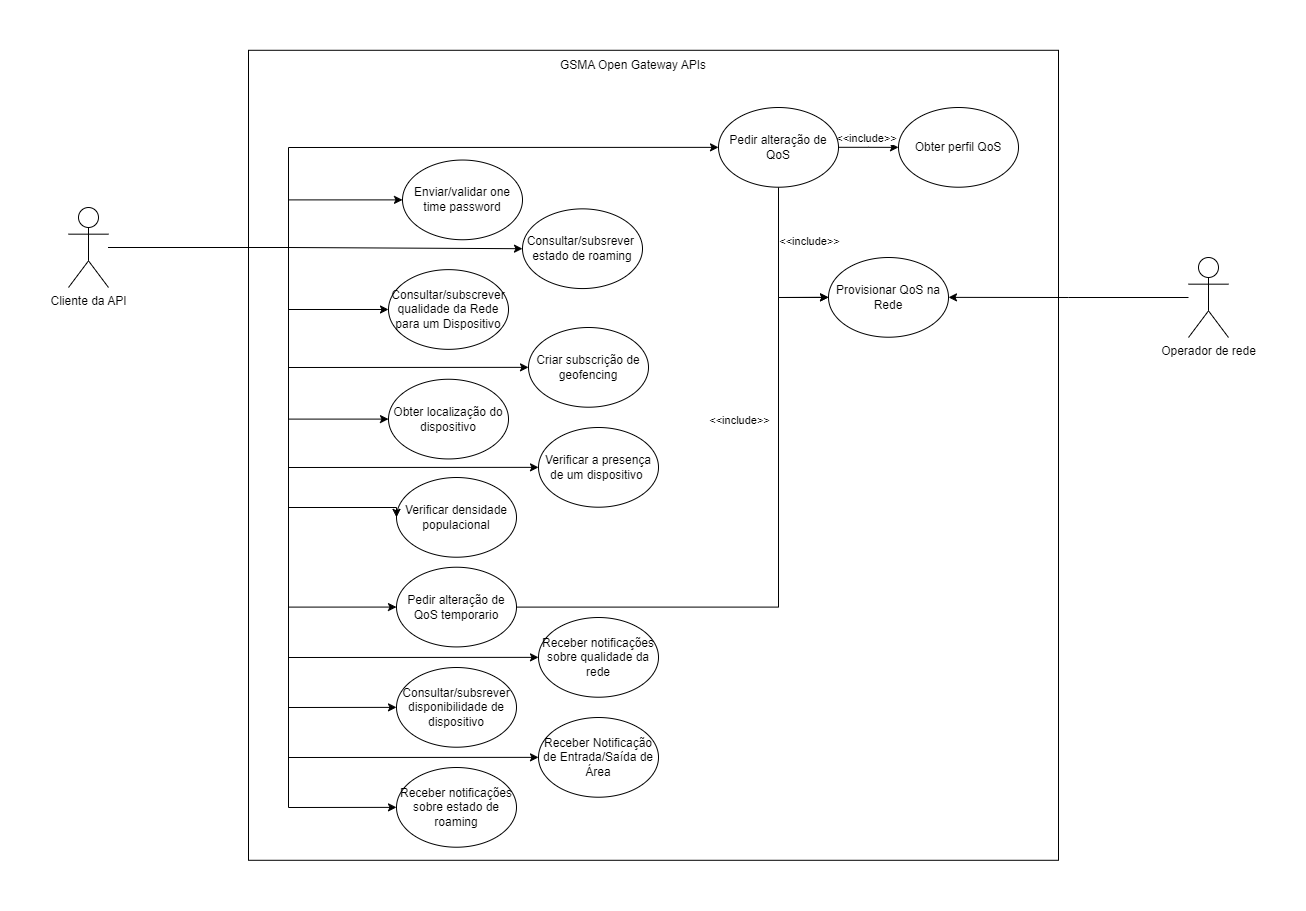
\includegraphics[width=20cm]{figs/use_case_diagram.png}
  }
  \caption{Diagrama de Casos de Uso}
\end{figure}

\begin{itemize}
  \item \textbf{Operador de rede}

    O operador de rede, apesar de poder interagir diretamente com
    o \emph{core 5G}, pode utilizar as APIs que disponibiliza para
    mais facilmente gerir a qualidade de serviço da sua rede

  \item{\textbf{Cliente da API}}

    Os clientes das APIs são os diversos negócios que pretendem
    programáticamente modificar a rede, ou para oferecer 
    melhores produtos/serviços aos seus clientes, ou para
    manipular uma rede interna para melhor se adaptar às suas
    necessidades.
    Utilizando as APIs definidas pelo \emph{GSMA Open Gateway},
    os diversos negócios podem:
    \begin{enumerate}
      \item Enviar/Validar One Time Passwords (OTPs), para 
        (por exemplo) verificar a validade de um número de telefone
        via SMS
      \item Consultar ou subscrever o estado do roaming, de modo a
        ser possível verificar se um dispositivo se encontra em
        outro país.
      \item Consultar e/ou subscrever a qualidade da rede para um
        determinado dispositivo, de modo a saber se os requisitos
        de rede para a aplicação podem ser alcançados, caso seja 
        subscrito, sempre que exista uma alteração na qualidade 
        será enviada uma notificação.

      \item Obter a localização de um dado dispositivo
      \item Verificar a presença de um dispositivo, isto é,
        verificar se um determinado dispositivo se encontra dentro 
        da área definida.
      \item Verificar a densidade populacional numa dada zona
      \item Pedir uma alteração de QoS, temporário ou não, devido à
        necessidade de uma largura de banda maior.
      \item Receber notificações sobre o estado da rede
      \item Receber notificações relativas à entrada ou saída de
        um dispositivo de uma dada área
      \item Subscrever/Consultar a disponibilidade de um
        dispositivo
    \end{enumerate}
\end{itemize}

\section{Requisitos}

Para o desenvolvimento do sistema foram recolhidos os diversos 
requisitos:

\subsection{Requisitos Funcionais}

\begin{itemize}
  \item \textbf{Serviços de Localização:}
    \begin{itemize}

      \item O sistema deve permitir a criação de assinaturas para que dispositivos recebam notificações ao entrar ou sair de uma área definida
      \item O sistema deve permitir a obtenção da localização de um dispositivo, sendo esta descrita por um círculo (coordenadas do centro e raio) ou um polígono simples (lista de coordenadas)
      \item O sistema deve permitir verificar se um dispositivo se encontra em uma certa área. Se esta área se encontra fora da área coberta pelo operador ou se esta área for válida, entre outros, deve retornar os erros corretos.
      \item O sistema deve permitir obter a estimativa da densidade populacional numa área especificada
    \end{itemize}

  \item \textbf{Qualidade de comunicação:}
    \begin{itemize}

      \item O sistema deve permitir a troca de informação relevante para auxiliar na tomada de decisões relacionadas às APIs da rede.
      \item O sistema deve permitir que desenvolvedores consultem a rede sobre a probabilidade de atender aos requisitos de conectividade numa sessão. 
      \item O sistema deve permitir que desenvolvedores possam definir diferentes QoS, nos AP dos clientes, dependendo da sua necessidade de largura de banda.
      \item O sistema deve permitir a obtenção dos perfis de QoS existentes numa rede, retornando assim a informação relativa aos mesmos.
      \item O sistema deve permitir a atribuição de perfis QoS a um dispositivo. A rede aplicará o perfil de QoS ao tráfego do dispositivo sempre que estiver conectado, até que este aprovisionamento seja removido.
    \end{itemize}

  \item \textbf{Proteção contra fraudes:}
    \begin{itemize}
      \item O sistema deve permitir a verificação de um número de telefone, através do envio e validação de uma OTP.
    \end{itemize}

  \item \textbf{Obtenção de informação sobre dispositivos:}
    \begin{itemize}

      \item O sistema deve permitir verificar se um determinado dispositivo está disponível na rede.
      \item O sistema deve permitir que um subscritor da API seja notificado caso exista uma alteração na disponibilidade de um determinado dispositivo.
      \item O sistema deve permitir verificar se um determinado dispositivo se encontra numa situação de roaming, caso isto seja verdade, retorna a informação existente sobre o país.
      \item O sistema deve permitir que um subscritor da API seja notificado caso exista alguma alteração no estado de roaming de um dispositivo.
    \end{itemize}
\end{itemize}

\subsection{Requisitos Não Funcionais}

\begin{itemize}
  \item \textbf{Desempenho e Latência:}
    \begin{itemize}
      \item O sistema deve manter tempos de resposta consistentes à medida que a base de utilizadores ou o volume de dados aumenta 
      \item O sistema deve conseguir tratar um número crescente de pedidos.
    \end{itemize}

  \item \textbf{Escalabilidade:}
    \begin{itemize}
      \item O sistema deve garantir que o sistema suporte um elevado volume de pedidos e dispositivos conectados
      \item O sistema deve escalar horizontalmente e/ou verticalmente consoante a procura.
    \end{itemize}

  \item \textbf{Disponibilidade e Fiabilidade:}
    \begin{itemize} 
      \item O sistema deve estabelecer níveis de disponibilidade (por exemplo, SLA de 99,9\% de uptime) 
      \item O sistema deve apresentar um nível de fiabilidade elevado (isto é, 99.9999\% de fiabilidade)
      \item O sistema deve ter um mecanismo de redundância e tolerância a falhas, garantindo a operação contínua mesmo em condições adversas.
    \end{itemize}
  \item  \textbf{Interoperabilidade:}
    \begin{itemize}
      \item O sistema deve ter compatibilidade com diversas operadoras, garantindo a integração das APIs com a infraestrutura de diferentes operadoras de rede, promovendo a universalidade dos serviços.
      \item O sistema deve assegurar que as APIs sigam padrões abertos e melhores práticas, promovendo a interoperabilidade e a aceitação universal entre os diversos sistemas e tecnologias.
    \end{itemize}


  \item \textbf{Manutenibilidade e Extensibilidade:}
    \begin{itemize}
      \item O sistema deve ter uma arquitetura modular, permitindo dividir o sistema em componentes independentes, facilitando atualizações e correções sem afetar o funcionamento global.
      \item O sistema deve ter uma documentação detalhada, com manuais, de modo a ajudar os desenvolvedores a compreender e manter o sistema eficazmente.
      \item O sistema deve ter código limpo e legível, seguindo padrões que tornam o código fácil de entender e modificar, reduzindo a probabilidade de erros.
      \item O sistema deve ter flexibilidade para atualizações, facilitando a implementação de novas funcionalidades ou melhorias sem a necessidade de reescrever grandes partes do código.
    \end{itemize}
  \item \textbf{Usabilidade:}
    \begin{itemize}
      \item O sistema deve retornar, caso existam, erros seguindo o padrão definido, facilitando a integração destas APIs.
      \item O sistema deve retornar somente a informação relevante ao desenvolvedor, abstraindo-o das informações mais complexas da rede
    \end{itemize}
\end{itemize}
